\documentclass{article}
\usepackage[utf8]{inputenc}
\usepackage[margin = 0.8in]{geometry}
\usepackage{graphicx}
\usepackage{amsmath, amssymb}
\usepackage{subcaption}
\usepackage{multirow}
\usepackage{mathtools}
\usepackage{float}


\title{RBE549 - Homework 3}
\author{Keith Chester}
\date{Due date: September 15, 2022}

\begin{document}
\maketitle

\section*{Problem 1}

In this problem we are applying dilation and then erosion using two different kernels.

\subsection*{A}

First, we apply our first kernel $S1$ to our input. We start by placing its kernel origin in the upper left corner.

\begin{figure}[H]
    \centering
    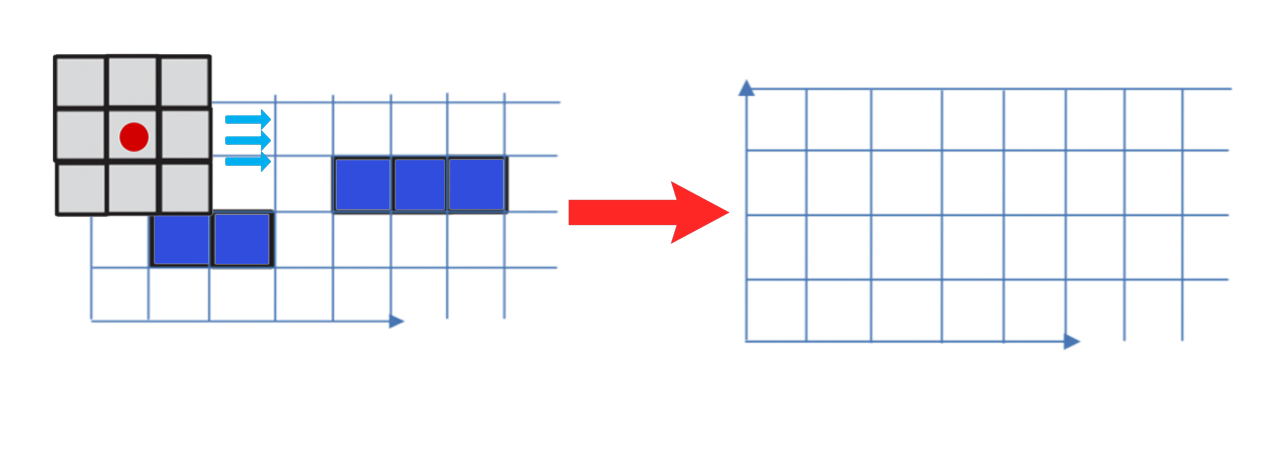
\includegraphics[width = 0.45\textwidth]{imgs/5/a1.png}
    \caption{Starting point}
    \label{fig:a1}
\end{figure}

The kernel then moves to the left. Since dilation is an $OR$ operation, as soon as our kernel encounters any $1$ value in the input image across the whole kernel, the point where the kernel origin is gets set to $1$.

\begin{figure}[H]
    \centering
    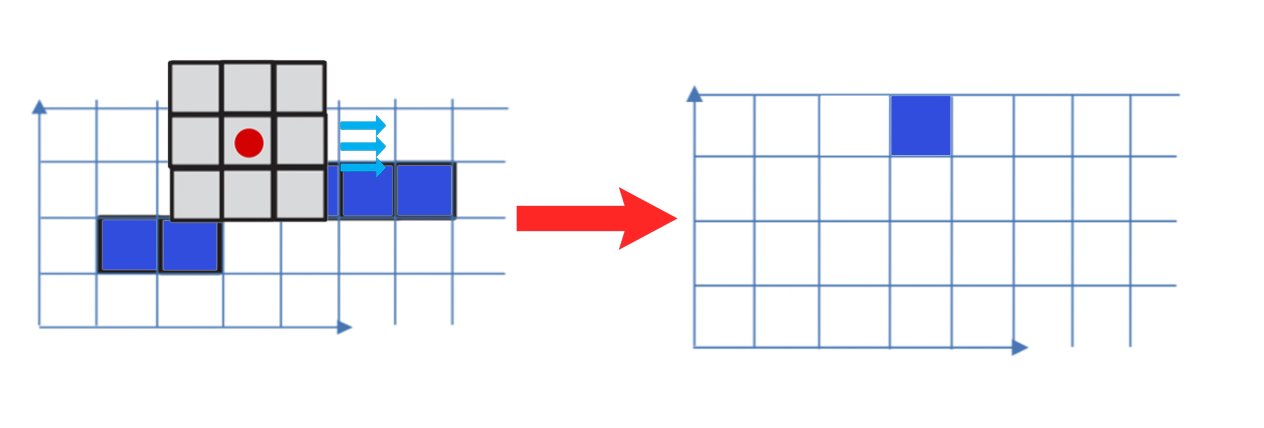
\includegraphics[width = 0.45\textwidth]{imgs/5/a2.png}
    \caption{First 1}
    \label{fig:a2}
\end{figure}

This continues until we hit our first edge with the kernel origin.

\begin{figure}[H]
    \centering
    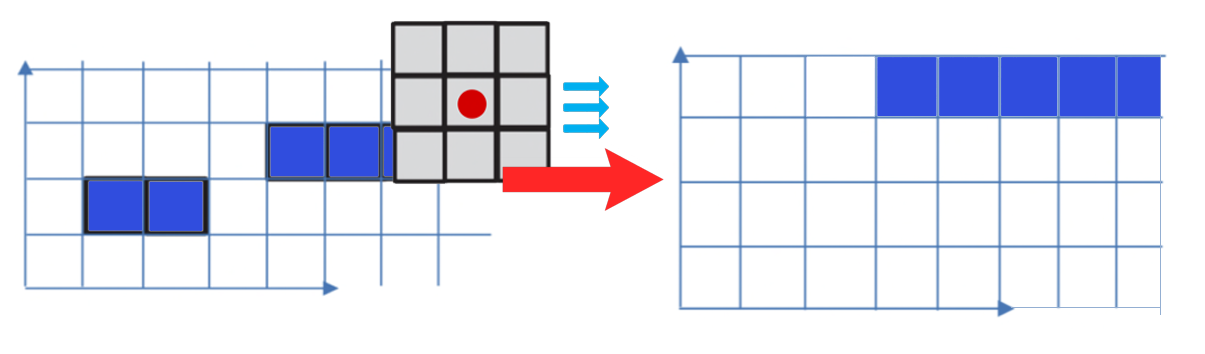
\includegraphics[width = 0.45\textwidth]{imgs/5/a3.png}
    \caption{First edge}
    \label{fig:a3}
\end{figure}

We then continue onto the next row.

\begin{figure}[H]
    \centering
    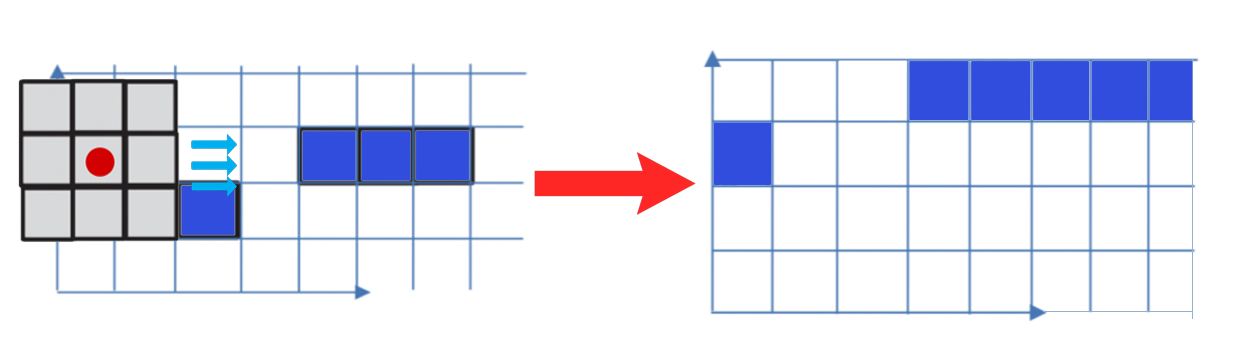
\includegraphics[width = 0.45\textwidth]{imgs/5/a4.png}
    \caption{Next row}
    \label{fig:a4}
\end{figure}

\begin{figure}[H]
    \centering
    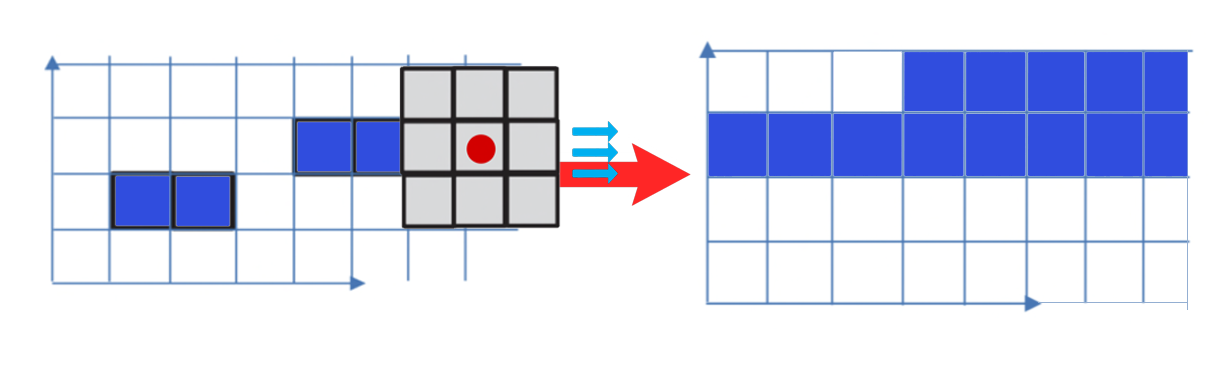
\includegraphics[width = 0.45\textwidth]{imgs/5/a5.png}
    \caption{Continuing the next row}
    \label{fig:a5}
\end{figure}

This continues until we reach our final point where the kernel no longer sees any $1$ values across the input image, and thus we begin to get a sequence of $0$'s across the bottom ending.

\begin{figure}[H]
    \centering
    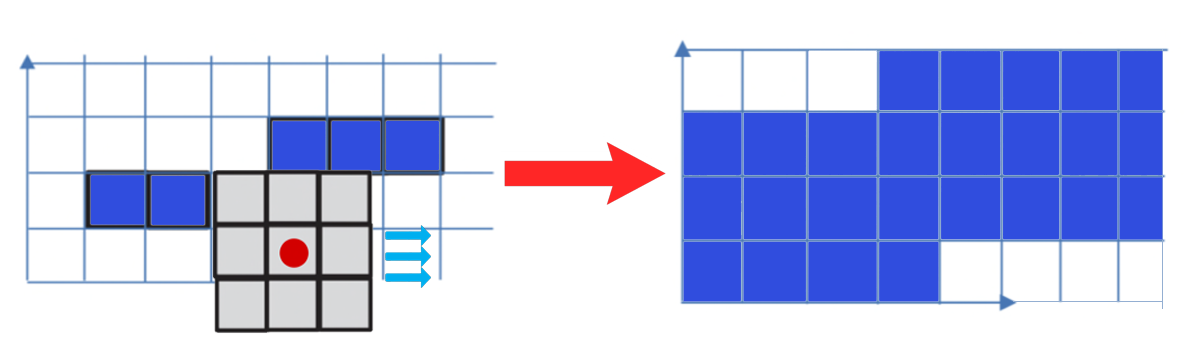
\includegraphics[width = 0.45\textwidth]{imgs/5/a6.png}
    \caption{Starting point}
    \label{fig:a6}
\end{figure}

This gives us the resulting dilation from the $S1$ kernel:

\begin{figure}[H]
    \centering
    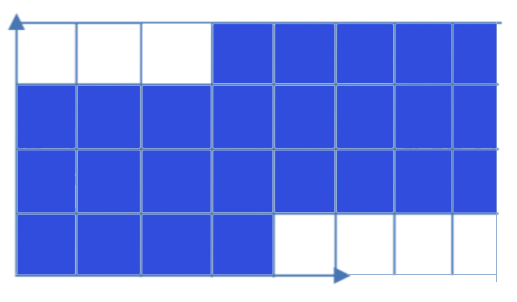
\includegraphics[width = 0.45\textwidth]{imgs/5/a7.png}
    \caption{A dilation result}
    \label{fig:a7}
\end{figure}

Now let's start applying erosion using kernel $S2$. It will move similarly across the image, but instead of an $OR$ operation it will be an $AND$ operation - thus if every active/$1$ (grey) square within the kernel does not fall upon a $1$ value within the input (our previous dilation) - then it will be set to $0$.

\begin{figure}[H]
    \centering
    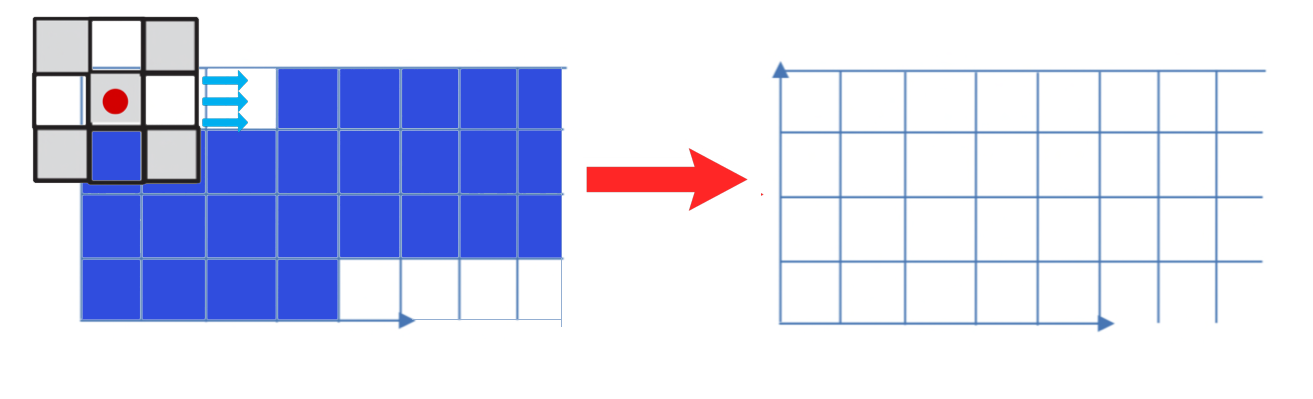
\includegraphics[width = 0.45\textwidth]{imgs/5/a8.png}
    \caption{Erosion starting point}
    \label{fig:a8}
\end{figure}

We move through, going across the row and finally moving down once we hit the end of the row, as before. The first point that we encounter a situation where \textit{all} of the $S2$ kernel's active points overlap a $1$.

\begin{figure}[H]
    \centering
    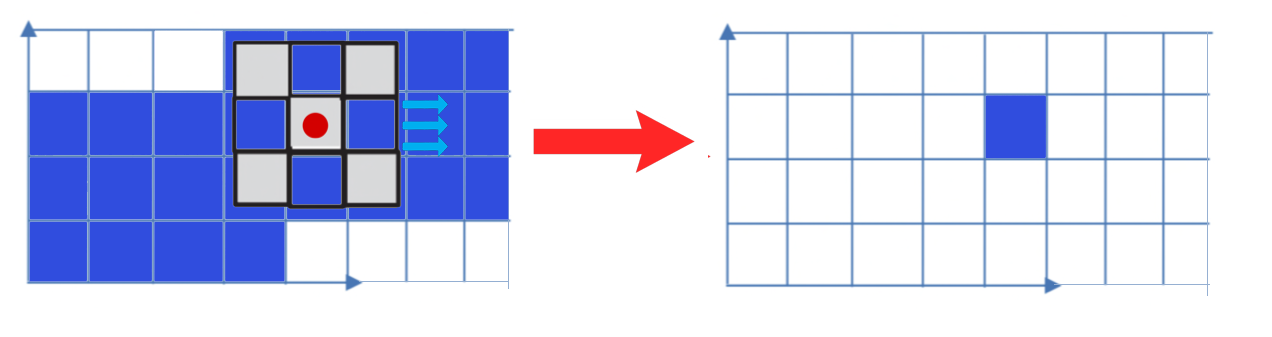
\includegraphics[width = 0.45\textwidth]{imgs/5/a9.png}
    \caption{Erosion first zero}
    \label{fig:a9}
\end{figure}

This continues on for the first row, but by the end we hit another area where our kernel does not hit all $1$s.

\begin{figure}[H]
    \centering
    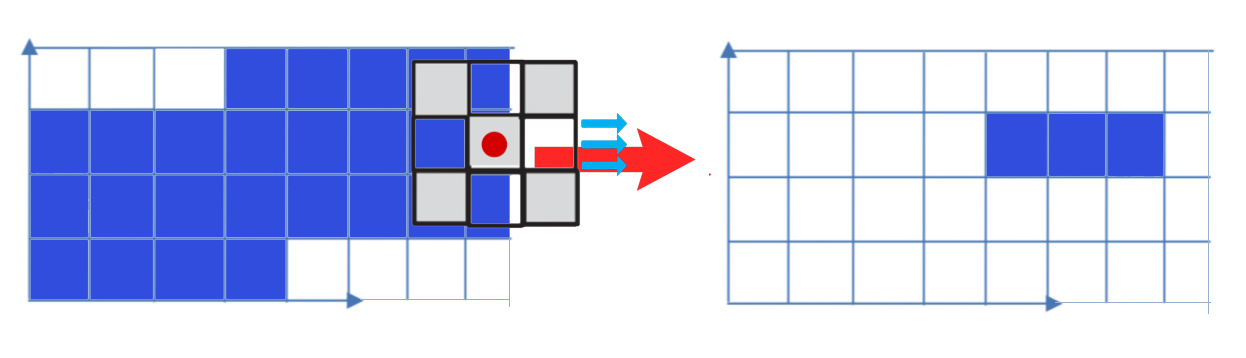
\includegraphics[width = 0.45\textwidth]{imgs/5/a10.png}
    \caption{Erosion first zero}
    \label{fig:a10}
\end{figure}

For the next row we begin to find more spots where we can mark the kernel orgin as $1$:

\begin{figure}[H]
    \centering
    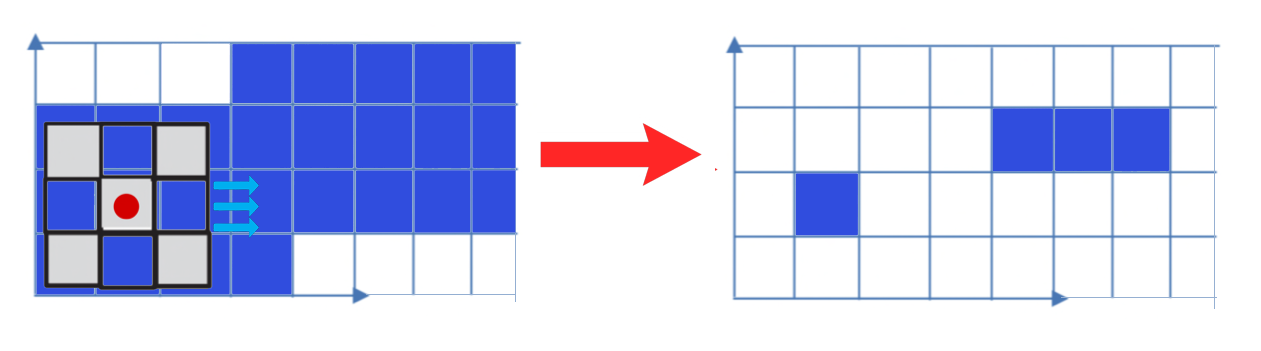
\includegraphics[width = 0.45\textwidth]{imgs/5/a11.png}
    \caption{Next row}
    \label{fig:a11}
\end{figure}

This continues for a few pixels until we reach a resulting $0$, which continues for the rest of the output.

\begin{figure}[H]
    \centering
    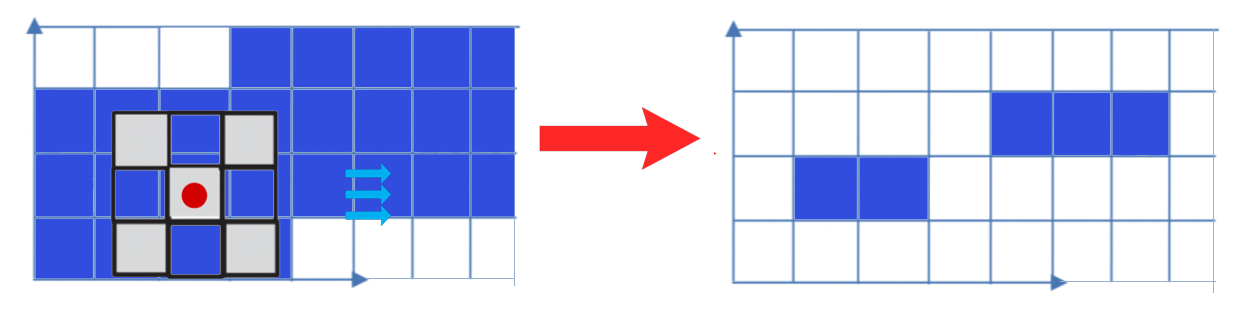
\includegraphics[width = 0.45\textwidth]{imgs/5/a12.png}
    \caption{Erosion continuing}
    \label{fig:a12}
\end{figure}

Our final result was:

\begin{figure}[H]
    \centering
    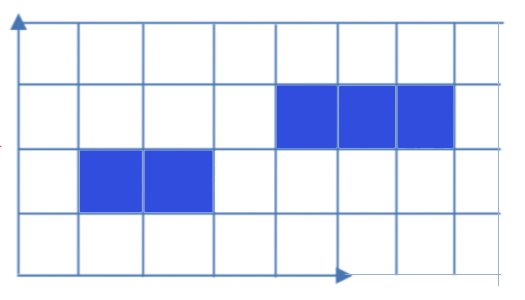
\includegraphics[width = 0.45\textwidth]{imgs/5/a13.png}
    \caption{Result}
    \label{fig:a13}
\end{figure}

\subsection*{B}

In this problem we also perform dilation and then erosion, but using kernel $S2$ for dilation and kernel $S1$ for erosion.

\begin{figure}[H]
    \centering
    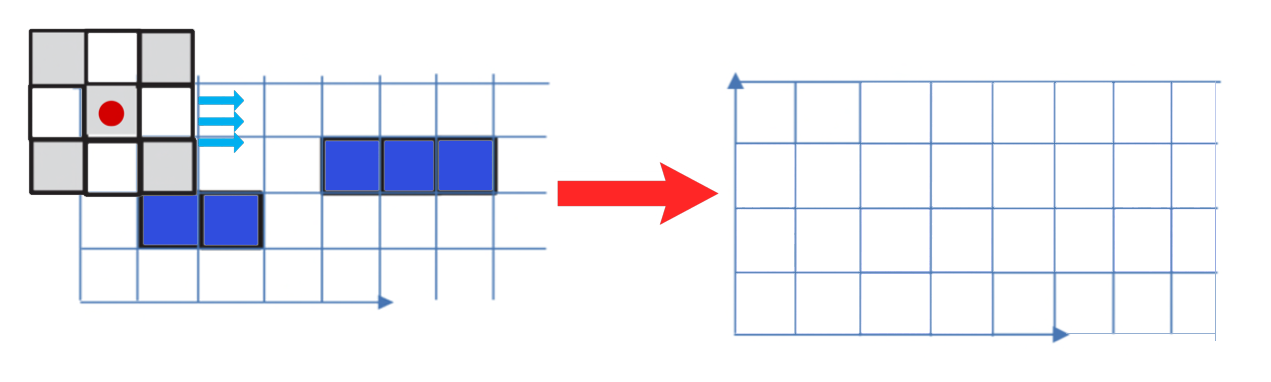
\includegraphics[width = 0.45\textwidth]{imgs/5/b1.png}
    \caption{Dilation starting point}
    \label{fig:b1}
\end{figure}

We begin as before, moving the kernel across. It is an $OR$ operation, so as long as any active piece of the kernel hits a $1$ the resulting kernel origin point on the output will be a $1$.

\begin{figure}[H]
    \centering
    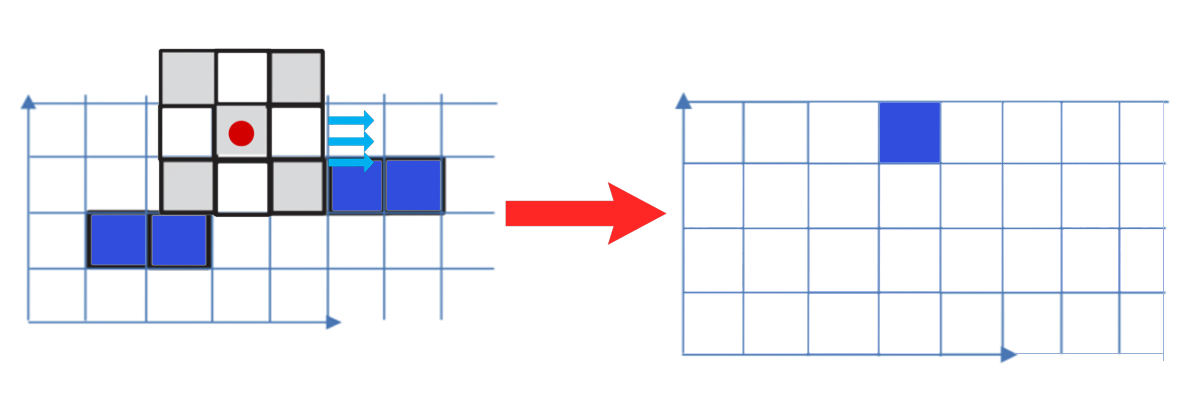
\includegraphics[width = 0.45\textwidth]{imgs/5/b2.png}
    \caption{First active point}
    \label{fig:b2}
\end{figure}

As before we go across to the end of the row, which has $1$s across the whole way from here.

\begin{figure}[H]
    \centering
    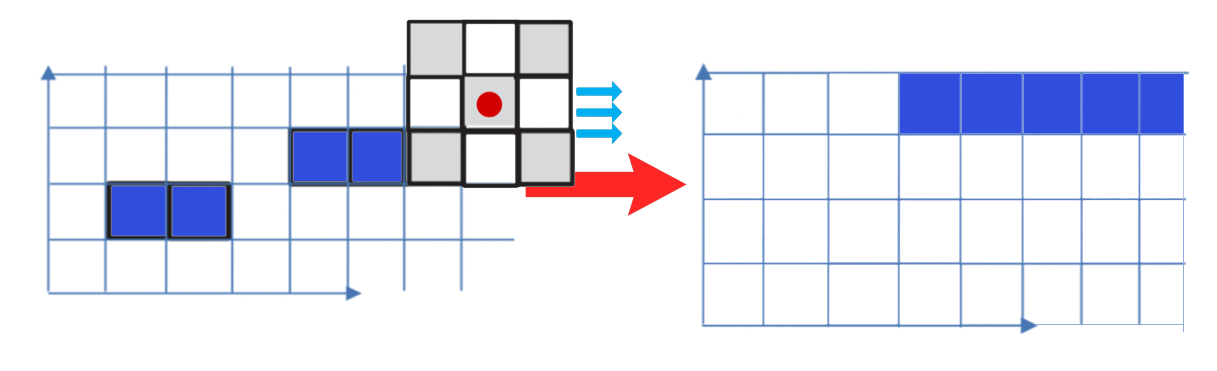
\includegraphics[width = 0.45\textwidth]{imgs/5/b3.png}
    \caption{Move to the end of the row}
    \label{fig:b3}
\end{figure}

...and then we move onto the next row as before.

\begin{figure}[H]
    \centering
    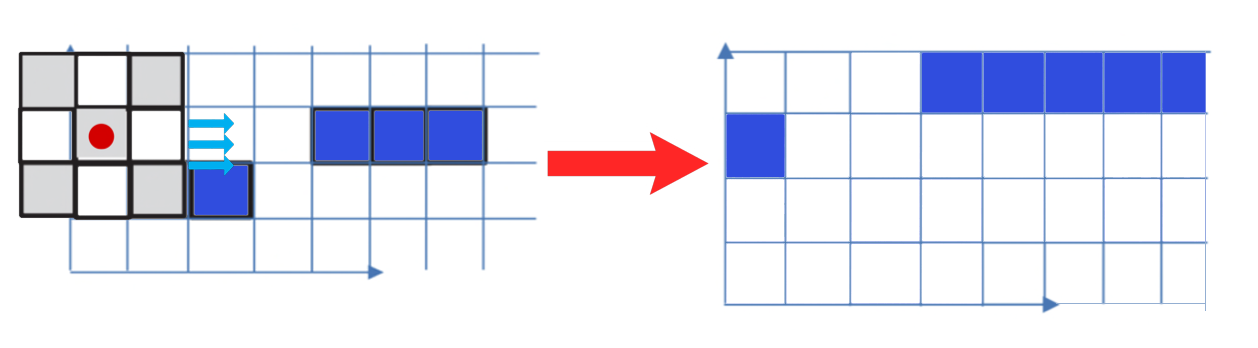
\includegraphics[width = 0.45\textwidth]{imgs/5/b4.png}
    \caption{Move onto the next row}
    \label{fig:b4}
\end{figure}

\begin{figure}[H]
    \centering
    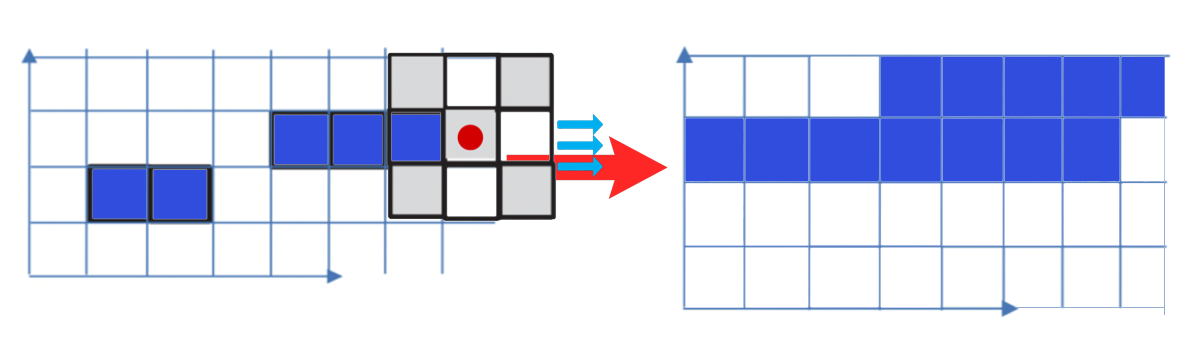
\includegraphics[width = 0.45\textwidth]{imgs/5/b5.png}
    \caption{End of that row}
    \label{fig:b5}
\end{figure}

At the start of the next row, we actuall find ourselves with $0$ results.

\begin{figure}[H]
    \centering
    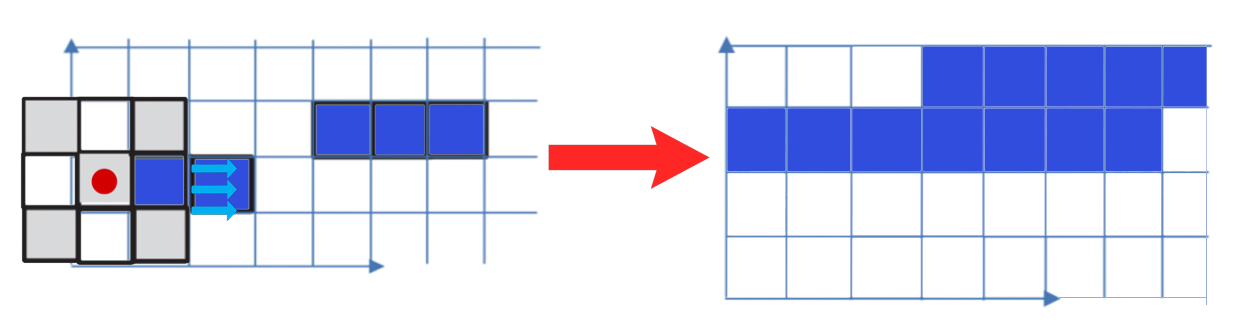
\includegraphics[width = 0.45\textwidth]{imgs/5/b6.png}
    \caption{Continuing to the next row}
    \label{fig:b6}
\end{figure}

This continues through as before...

\begin{figure}[H]
    \centering
    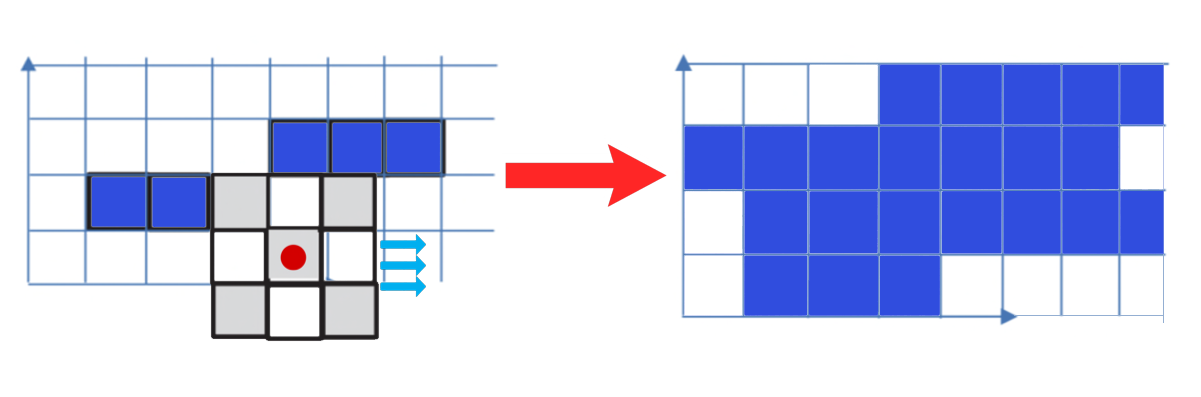
\includegraphics[width = 0.45\textwidth]{imgs/5/b7.png}
    \caption{Moving through to the end}
    \label{fig:b7}
\end{figure}

...resulting in this final dilation result.

\begin{figure}[H]
    \centering
    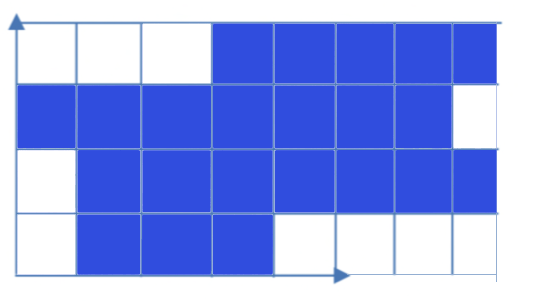
\includegraphics[width = 0.45\textwidth]{imgs/5/b8.png}
    \caption{Dilation result}
    \label{fig:b8}
\end{figure}

We then use the $S1$ kernel to apply erosion, which again, is an $AND$ operation, requiring that all points of the kernel overlap on a $1$ value on the input (our dilation output).

\begin{figure}[H]
    \centering
    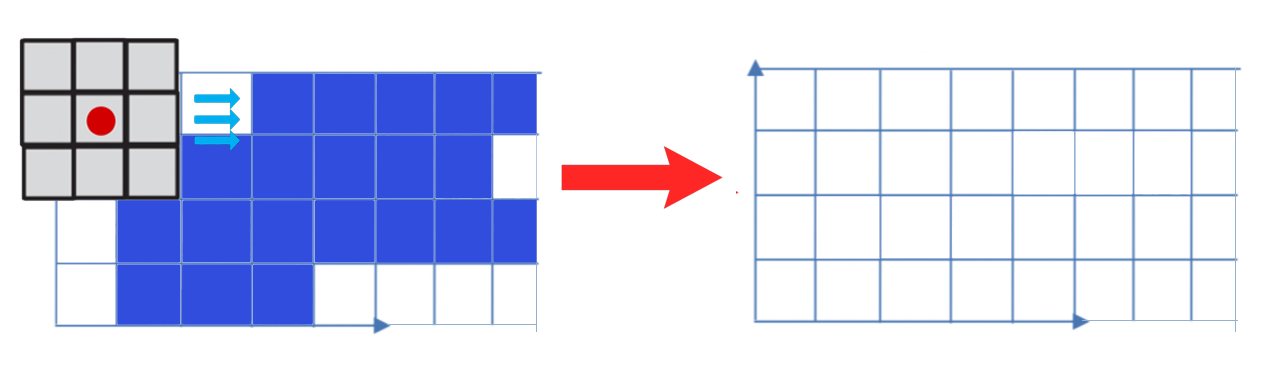
\includegraphics[width = 0.45\textwidth]{imgs/5/b9.png}
    \caption{Erosion starting point}
    \label{fig:b9}
\end{figure}

The erosion moves through, activating only a few times on the second row.

\begin{figure}[H]
    \centering
    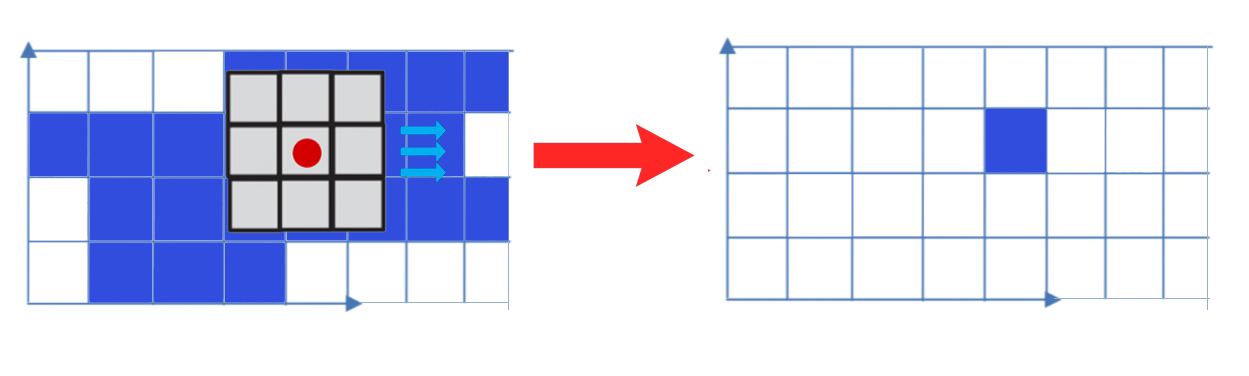
\includegraphics[width = 0.45\textwidth]{imgs/5/b10.png}
    \caption{First point marked $1$ with erosion}
    \label{fig:b10}
\end{figure}

\begin{figure}[H]
    \centering
    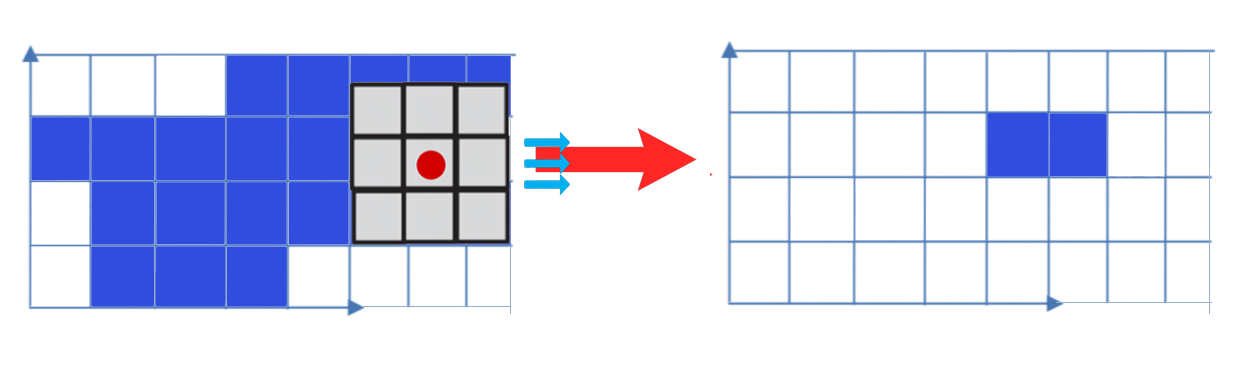
\includegraphics[width = 0.45\textwidth]{imgs/5/b11.png}
    \caption{Moving through the second row with erosion}
    \label{fig:b11}
\end{figure}

The erosion kernel then moves through and finds the only point on the third row (and final point overall) that receies a $1$ value.

\begin{figure}[H]
    \centering
    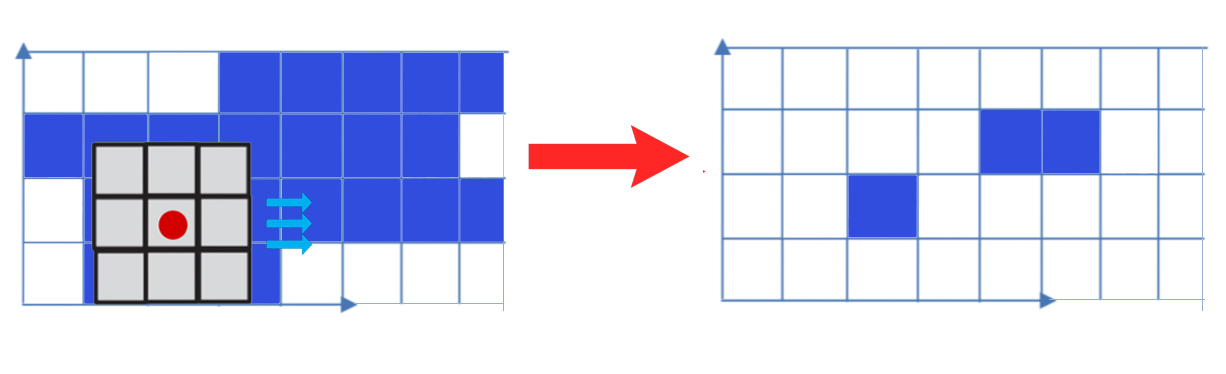
\includegraphics[width = 0.45\textwidth]{imgs/5/b12.png}
    \caption{Erosion result}
    \label{fig:b12}
\end{figure}

This gives us the final result of:

\begin{figure}[H]
    \centering
    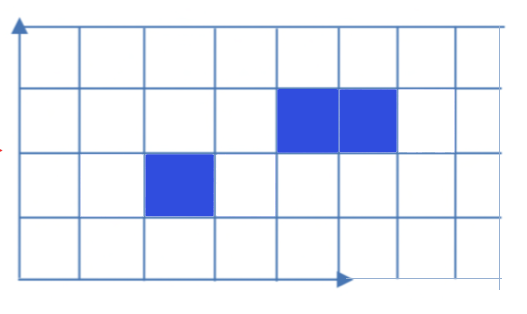
\includegraphics[width = 0.45\textwidth]{imgs/5/b13.png}
    \caption{Dilation starting point}
    \label{fig:b13}
\end{figure}

\section*{Problem 2}

For this problem, we are attempting to prove the associative property of convolution:

\begin{equation}
    f(\vec{x})*(g(\vec{x})*h(\vec{x})) = (f(\vec{x})*g(\vec{x}))*h(\vec{x})
\end{equation}

first we will define additional functions $y_1(\vec{x})$ and $y_2(\vec{x})$, such that:

\begin{equation}
    f(\vec{x})*y_1(\vec{x}) = y_2(\vec{x})*h(\vec{x})
\end{equation}

We then begin expanding the definition of $y_n(\vec{x})$ via the definition of convolution:

\begin{equation}
    y_1(\vec{x}) = \sum^\infty_{i=-\infty} g(i) h(\vec{x}-i)
\end{equation}

\begin{equation}
    y_2(\vec{x}) = \sum^\infty_{i=-\infty} f(i) g(\vec{x}-i)
\end{equation}

...then we start looking deeper into $y_2$:

\begin{equation}
    =\sum^\infty_{k=-\infty} y_2(k) h(\vec{x}-k)
\end{equation}

\begin{equation}
    =\sum^\infty_{k=-\infty} \sum^\infty_{i=-\infty} f(i) g(\vec{x}-i) h(\vec{x}-k)
\end{equation}

\begin{equation}
    =\sum^\infty_{i=-\infty}f(i) \sum^{\infty}_{k=-\infty} g(k-i) h(\vec{x}-k)
\end{equation}

To simplify, we're going to define a new variable $j$, where $j=k-i$, or $k=j+i$:

\begin{equation}
    =\sum^\infty_{i=-\infty} f(i) \sum^\infty_{k=-\infty} g(j) h(\vec{x}-j-i)
\end{equation}

Looking back to $y_1$...

\begin{equation}
    y_1(\vec{x}-i) = \sum^\infty_{j=-\infty} g(j) h(\vec{x}-i-j)
\end{equation}

These are similar to what we saw in the prior equation. We can thus expand:

\begin{equation}
    \sum^\infty_{i=-\infty} f(i) y_1(\vec{x}-i)
\end{equation}

\begin{equation}
    = f (\vec{x}) * y_1 (\vec{x})
\end{equation}

\begin{equation}
    =f(\vec{x})*(g(\vec{x})*h(\vec{x}))
\end{equation}

...which matches the other side. Therefore, we have shown that convolution's associative property is true.

\section*{Problem 3}

In this question we are are tasked with finding the Discrete Fourier Transform for a simple x-direction mask, with a kernel of $[1, -1]$ with $1$ being our kernel origin. We will be using the 1-D DFT formula:

\begin{equation}
    H(k) = \sum^{N-1}_{x=0} h(x)e^{-j\frac{2\pi k x}{N}}
\end{equation}

First, we define set constants from this problem as proposed. $N=2$, $h(0)=1$, and $h(1) = -1$. With this we can begin to simplify the equation:

\begin{equation}
    H(k) = \sum^{1}_{x=0} h(x)e^{-j \pi k x}
\end{equation}

\begin{equation}
    H(k) = h(0)e^{-j \pi k (0)} + h(1)e^{-j \pi k (1)}
\end{equation}

\begin{equation}
    H(k) = e ^ 0 - e^{-j\pi k}
\end{equation}

\begin{equation}
    H(k) = 1 - e^{-j \pi k}
\end{equation}

Using an identity, we know that $e^{AB} = \cos{B} + A\sin{B}$. Thus:

\begin{equation}
    H(k) = 1 - \cos{k\pi} + j \sin{k\pi}
\end{equation}

This should be our DFT for the provided kernel.

\section*{Problem 4}

In this problem, we aim to utilize the popular OpenCV framework in Python to demonstrate image smoothing through a few common approaches. Specifically, we will be showing a box filter, a Gaussian filter, and a median filter with specified settings. The application of those filters can be demonstrated below, and the code can be ran to show each of these filters being applied by running this homework's associated \textit{problem5.py}.

\begin{figure}[H]
    \centering
    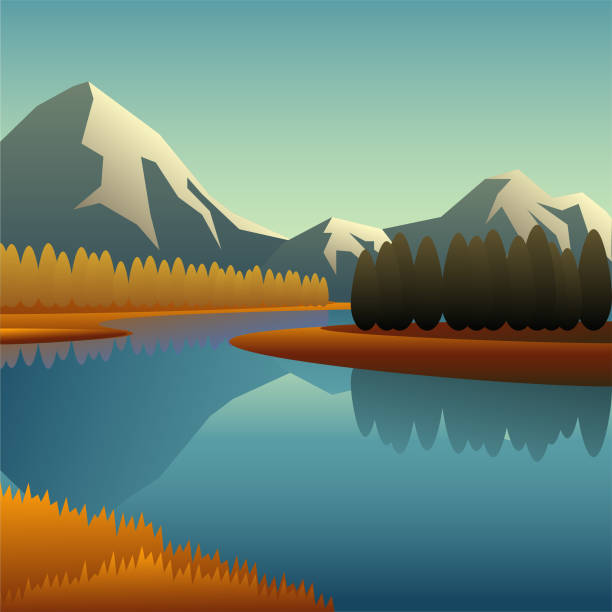
\includegraphics[width = 0.45\textwidth]{imgs/artwork.jpg}
    \caption{The unmodified artwork}
    \label{fig:base_image}
\end{figure}

\begin{figure}[H]
    \centering
    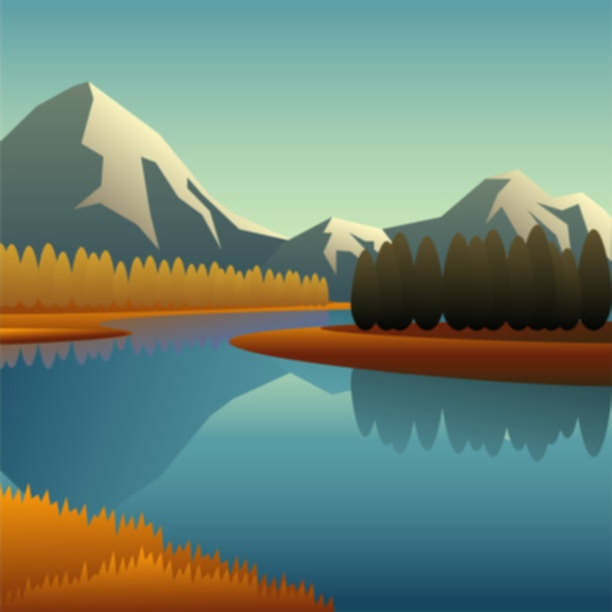
\includegraphics[width = 0.45\textwidth]{imgs/box_filtered_artwork.jpg}
    \caption{Box Filter}
    \label{fig:box_filter}
\end{figure}

\begin{figure}[H]
    \centering
    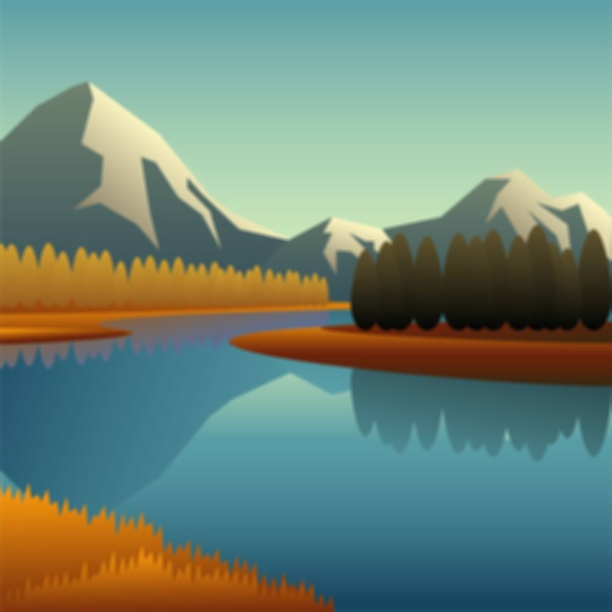
\includegraphics[width = 0.45\textwidth]{imgs/gaussian_artwork.jpg}
    \caption{Gaussian Filter}
    \label{fig:gaussian}
\end{figure}

\begin{figure}[H]
    \centering
    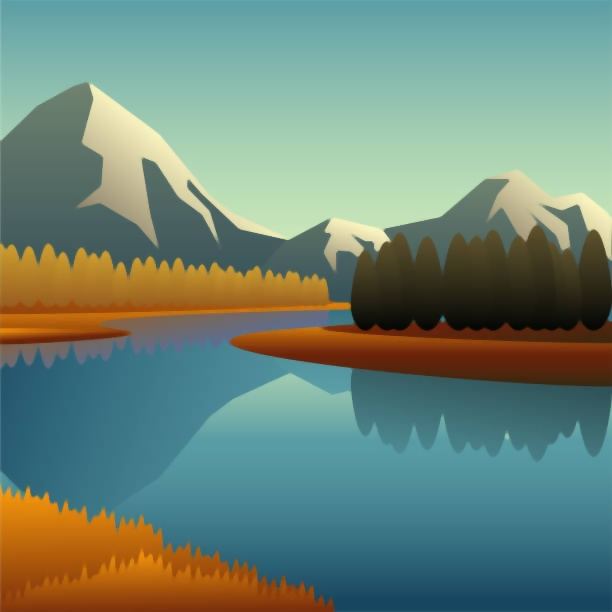
\includegraphics[width = 0.45\textwidth]{imgs/median_artwork.jpg}
    \caption{Median Filter}
    \label{fig:median}
\end{figure}

Throughout these pictures, we can see the different effects of blurring across each image once the filter is applied. The Gaussian seems to blur outwards from edges of shapes, the median blur a softening of the photo without losing information from its edges, and the box filter loses some finer details of what was in the original image.

In the second part of our question, we were asked what happens if we change the window size? We explored that in the second half of the code within \textit{problem5.py}, and the results are shown below. We tripled the size of each parameter from the prior part of this problem.

\begin{figure}[H]
    \centering
    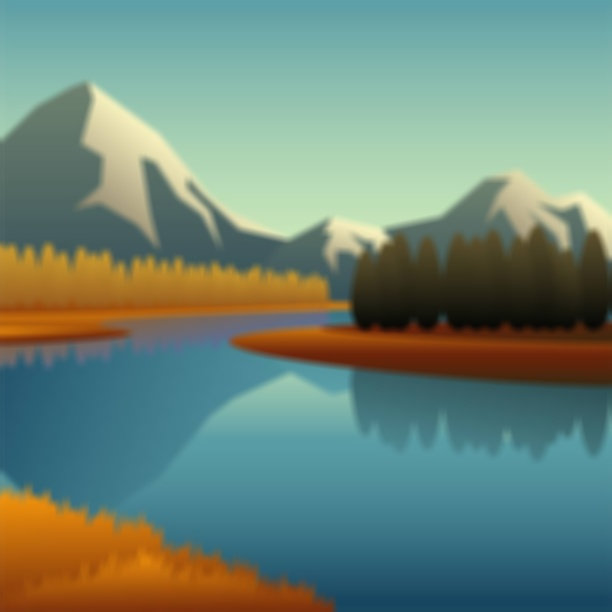
\includegraphics[width = 0.45\textwidth]{imgs/3x_box_filtered_artwork.jpg}
    \caption{Box Filter at $W=9$}
    \label{fig:3x_box}
\end{figure}

\begin{figure}[H]
    \centering
    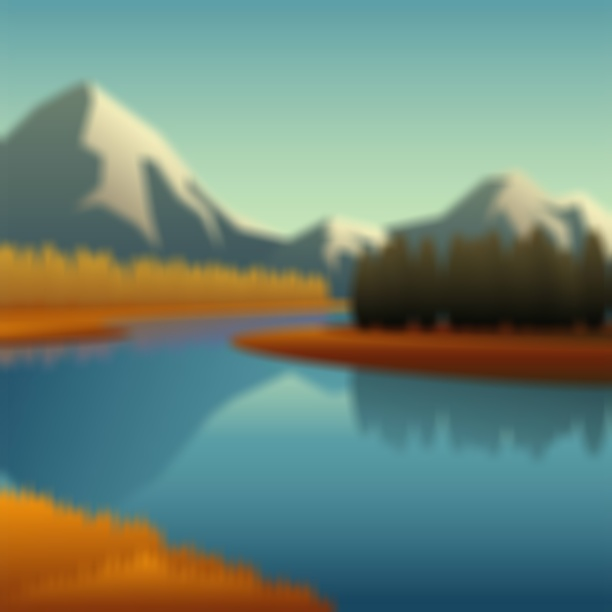
\includegraphics[width = 0.45\textwidth]{imgs/3x_gaussian_artwork.jpg}
    \caption{Gaussian Filter at $\sigma=15$}
    \label{fig:3x_gaussian}
\end{figure}

\begin{figure}[H]
    \centering
    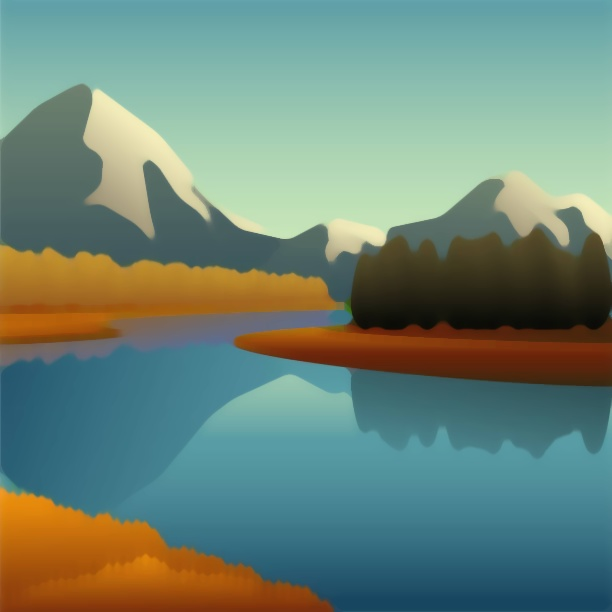
\includegraphics[width = 0.45\textwidth]{imgs/3x_median_artwork.jpg}
    \caption{Median Filter with a 15x15 filter}
    \label{fig:3x_median}
\end{figure}

Here we see the box filter lose more detail, but maintain edge definition. The Gaussian blur becomes unfocused with edges becoming far less defined and ultimately being lost within the forest. The median filter does see slightly more blurring, but far less of a change than previous filters.

\end{document}